% Standalone Crop of the Agricultural System Flow Diagram
% SPDX-License-Identifier: Apache-2.0
\documentclass[tikz,border=6pt]{standalone}
\usepackage[T1]{fontenc}
\usepackage{lmodern}
\usetikzlibrary{shapes.geometric,arrows.meta,positioning,calc,fit,backgrounds}

% Curated Palette for Agricultural Intelligence System
\definecolor{containerBorder}{RGB}{165, 180, 205}
\definecolor{containerBg}{RGB}{252, 253, 255}
\definecolor{nodeBorder}{RGB}{65, 75, 90}
\definecolor{nodeBg}{RGB}{255, 255, 255}
\definecolor{diamondBorder}{RGB}{180, 85, 50}
\definecolor{diamondBg}{RGB}{255, 248, 242}
\definecolor{arrowColor}{RGB}{45, 55, 70}
\definecolor{titleText}{RGB}{25, 40, 60}

\begin{document}
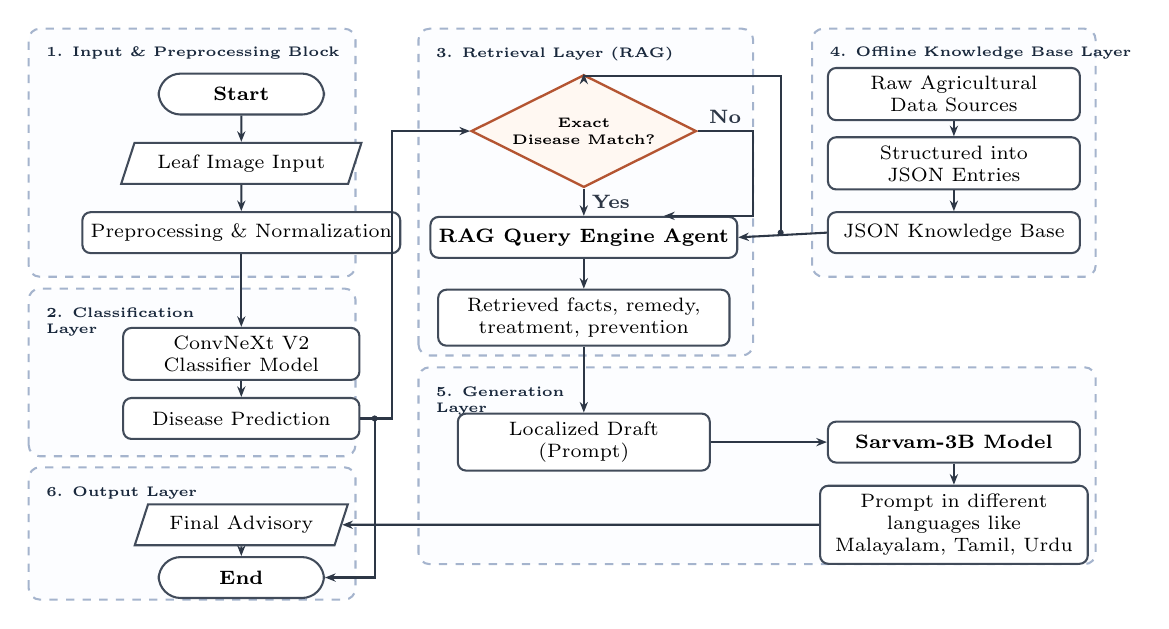
\begin{tikzpicture}[
    x=1cm, y=1cm,
    font=\sffamily,
    % Node styles
    terminal/.style={
        rectangle,
        rounded corners=8pt,
        draw=nodeBorder,
        fill=nodeBg,
        line width=0.75pt,
        minimum width=2.1cm,
        minimum height=0.52cm,
        align=center,
        font=\scriptsize\bfseries
    },
    io_node/.style={
        trapezium,
        trapezium left angle=72,
        trapezium right angle=108,
        draw=nodeBorder,
        fill=nodeBg,
        line width=0.75pt,
        minimum width=2.7cm,
        minimum height=0.52cm,
        align=center,
        font=\scriptsize
    },
    proc_node/.style={
        rectangle,
        rounded corners=3pt,
        draw=nodeBorder,
        fill=nodeBg,
        line width=0.75pt,
        minimum width=3.0cm,
        minimum height=0.52cm,
        align=center,
        font=\scriptsize,
        inner sep=3pt
    },
    decision/.style={
        diamond,
        aspect=2.0,
        draw=diamondBorder,
        fill=diamondBg,
        line width=0.85pt,
        align=center,
        font=\tiny\bfseries,
        inner sep=1.8pt
    },
    container/.style={
        draw=containerBorder,
        fill=containerBg,
        line width=0.75pt,
        dashed,
        rounded corners=4pt
    },
    layer_title/.style={
        font=\tiny\bfseries,
        text=titleText,
        anchor=north west,
        align=left
    },
    flow/.style={
        -{Stealth[scale=0.85, length=4.5pt, width=3.5pt]},
        line width=0.75pt,
        draw=arrowColor
    },
    label_text/.style={
        font=\scriptsize\bfseries,
        fill=containerBg,
        inner sep=1.5pt,
        text=arrowColor
    }
]

    % =========================================================================
    % BACKGROUND CONTAINERS (Exact geometry, zero overlapping)
    % =========================================================================
    \begin{scope}[on background layer]
        % 1. Input & Preprocessing Block
        \draw [container] (-6.35, 0.10) rectangle (-2.20, 3.25);
        \node [layer_title] at (-6.25, 3.14) {1. Input \& Preprocessing Block};

        % 2. Classification Layer
        \draw [container] (-6.35, -2.18) rectangle (-2.20, -0.05);
        \node [layer_title] at (-6.25, -0.17) {2. Classification\\Layer};

        % 6. Output Layer
        \draw [container] (-6.35, -4.00) rectangle (-2.20, -2.32);
        \node [layer_title] at (-6.25, -2.44) {6. Output Layer};

        % 3. Retrieval Layer (RAG)
        \draw [container] (-1.40, -0.90) rectangle (2.85, 3.25);
        \node [layer_title] at (-1.30, 3.14) {3. Retrieval Layer (RAG)};

        % 4. Offline Knowledge Base Layer
        \draw [container] (3.60, 0.10) rectangle (7.20, 3.25);
        \node [layer_title] at (3.70, 3.14) {4. Offline Knowledge Base Layer};

        % 5. Generation Layer
        \draw [container] (-1.40, -3.55) rectangle (7.20, -1.05);
        \node [layer_title] at (-1.30, -1.17) {5. Generation\\Layer};
    \end{scope}

    % =========================================================================
    % NODES
    % =========================================================================

    % --- Column 1: Input & Preprocessing (Centered at X = -3.65) ---
    \node [terminal] (start) at (-3.65, 2.42) {Start};
    \node [io_node] (img_input) at (-3.65, 1.54) {Leaf Image Input};
    \node [proc_node] (preprocess) at (-3.65, 0.66) {Preprocessing \& Normalization};

    % --- Column 1: Classification ---
    \node [proc_node] (convnext) at (-3.65, -0.88) {ConvNeXt V2\\Classifier Model};
    \node [proc_node] (pred) at (-3.65, -1.70) {Disease Prediction};

    % --- Column 1: Output ---
    \node [io_node] (advisory) at (-3.65, -3.05) {Final Advisory};
    \node [terminal] (end_node) at (-3.65, -3.72) {End};

    % --- Column 2: Retrieval Layer (RAG) (Centered at X = 0.70) ---
    \node [decision] (match) at (0.70, 1.95) {Exact\\Disease Match?};
    \node [proc_node, minimum width=3.7cm] (rag_engine) at (0.70, 0.60) {\textbf{RAG Query Engine Agent}};
    \node [proc_node, minimum width=3.7cm] (facts) at (0.70, -0.42) {Retrieved facts, remedy,\\treatment, prevention};

    % --- Column 3: Offline Knowledge Base Layer (Centered at X = 5.40) ---
    \node [proc_node, minimum width=3.2cm] (raw_data) at (5.40, 2.42) {Raw Agricultural\\Data Sources};
    \node [proc_node, minimum width=3.2cm] (json_struct) at (5.40, 1.54) {Structured into\\JSON Entries};
    \node [proc_node, minimum width=3.2cm] (json_kb) at (5.40, 0.66) {JSON Knowledge Base};

    % --- Column 2 & 3: Generation Layer ---
    \node [proc_node, minimum width=3.2cm] (draft) at (0.70, -2.00) {Localized Draft\\(Prompt)};
    \node [proc_node, minimum width=3.2cm] (sarvam) at (5.40, -2.00) {\textbf{Sarvam-3B Model}};
    \node [proc_node, minimum width=3.4cm] (multilingual) at (5.40, -3.05) {Prompt in different\\languages like\\Malayalam, Tamil, Urdu};

    % =========================================================================
    % CONNECTING ARROWS (Orthogonal, collision-free)
    % =========================================================================

    % Block 1 Intra-flow
    \draw [flow] (start) -- (img_input);
    \draw [flow] (img_input) -- (preprocess);

    % Block 1 to Block 2
    \draw [flow] (preprocess) -- (convnext);

    % Block 2 Intra-flow
    \draw [flow] (convnext) -- (pred);

    % Block 2 to Block 3 (Prediction -> Exact Disease Match?)
    % Routes through dedicated vertical channel at X = -1.75
    \draw [flow] (pred.east) -- ++(0.40, 0) coordinate (p_match) -- (p_match |- match.west) -- (match.west);

    % Alternate Unidentifiable / Low-confidence fallback to End
    % Routes parallel in channel at X = -1.98
    \draw [flow] (pred.east) ++(0.18, 0) coordinate (p_alt) -- (p_alt |- end_node.east) -- (end_node.east);
    \fill [arrowColor] (p_alt) circle (1.1pt);

    % Block 3: Yes / No Branches
    \draw [flow] (match.south) -- node [label_text, right=1pt] {Yes} (rag_engine.north);
    \draw [flow] (match.east) -- node [label_text, above=1pt] {No} ++(0.7, 0) coordinate (p_no) -- (p_no |- rag_engine.15) -- (rag_engine.15);

    % Block 4 Intra-flow
    \draw [flow] (raw_data) -- (json_struct);
    \draw [flow] (json_struct) -- (json_kb);

    % Block 4 Knowledge Base to RAG Engine (clean horizontal)
    \draw [flow] (json_kb.west) -- (rag_engine.east);

    % Taxonomy validation link up into top of match diamond
    % Routes cleanly at X = 3.20, then across at Y = 2.65 (below layer title, above diamond)
    \draw [flow] (3.20, 0.66) -- (3.20, 2.65) -- (match.north |- 0, 2.65) -- (match.north);
    \fill [arrowColor] (3.20, 0.66) circle (1.1pt);

    % Block 3 to Block 5
    \draw [flow] (rag_engine) -- (facts);
    \draw [flow] (facts) -- (draft);

    % Block 5 Intra-flow
    \draw [flow] (draft) -- (sarvam);
    \draw [flow] (sarvam) -- (multilingual);

    % Block 5 to Block 6: Multilingual prompt to Final Advisory (pure horizontal)
    \draw [flow] (multilingual.west) -- (advisory.east);

    % Block 6 Intra-flow
    \draw [flow] (advisory) -- (end_node);

\end{tikzpicture}
\end{document}
